
\section{Text past this point needs to be rewritten}
\subsubsection{The layer editor}
To set up and edit the vertical device structure, use the layer editor this is shown in figure \ref{fig:layer_editor}. Using this tool, you can add layers, remove layers, and move layers up and down.
\linebreak
\linebreak 
\textbf{The first column}: This is a human readable name for the layer.
\linebreak 
\linebreak 
\textbf{The second column}: The thickness of the layer in meters.
\linebreak
\linebreak 
\textbf{Third column}: Sets the optical material properties.
\linebreak
\linebreak 
\textbf{Forth column}: Sets how the model treats the layer.  The optical equations are solved over all layers.  However, if the layer is set as 'active layer', then gpvdm will the also solve the electrical equations over this layer.  More than one layer can be set as an active layer, in this case, the electrical equations will be solved over all, the layers marked 'active layer', this is useful when simulating heterojunctions.  A layer type 'other', means that the electrical equations will not be solved over that layer, but the optical equations will be.  A layer type contact, denotes that the layer represents a contact layer.  This is only affects/is needed for 2/3D simulations.


\begin{figure}[ht!]
\centering
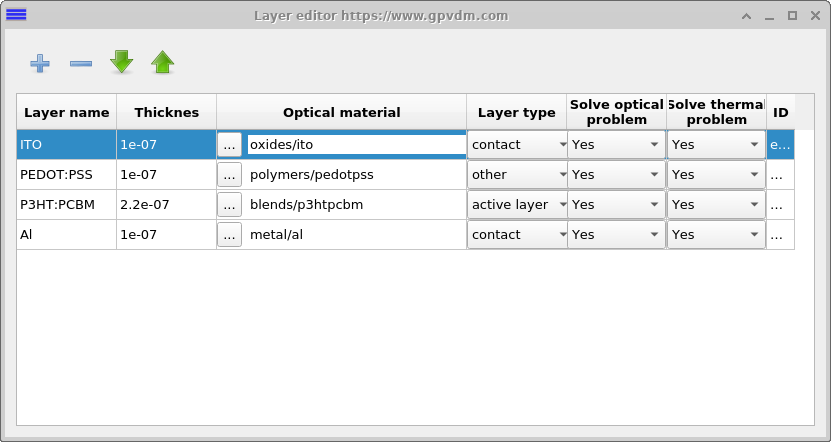
\includegraphics[width=\textwidth]{./images/layer_editor.png}
{\caption{The contact editor.}}
\label{fig:layer_editor}
\end{figure}

\subsubsection{The contact editor}

The contact editor is used to edit the contacts on the device, and what voltages are applied to which contacts, see figure \ref{fig:contact_editor}.  For a 1D simulation you can pretty much ignore this window.
\linebreak
\linebreak 
\textbf{The first column}: The human readable name for the contact.
\linebreak 
\linebreak 
\textbf{The second column}: Sets if the contact is at the top or bottom of the device.  There should be at least one contact at the top and one contact at the bottom of the device.  Some devices (OFETs) can have more than one contact at the top of the device. 
\linebreak
\linebreak 
\textbf{Third column}: This sets if the contact is 'active'.  In it's simplest form, an active contact is the contact to which the voltage ramp is applied during a JV curve simulation.  In a JV curve simulation, one contact will be held at 0 volts, while a steadily increasing voltage is applied to the other 'active' contact of the device.  If you are performing a transient voltage simulation, such as CELIV, the 'active' contact will have the CELIV voltage transient applied to it.  Swapping around the active contacts is equivalent to picking up the diode and turning it through 180 degrees and placing it back in the circuit.  This feature is most useful, when simulating OFETs, when one wants to apply a voltage ramp to one contact (i.e. the gate) out of three or four.
\linebreak
\linebreak 
\textbf{Forth column}: The start of the contact, not used in 1D simulations
\linebreak
\linebreak 
\textbf{Fifth column}: The width of the contact, not used in 1D simulations.
\linebreak
\linebreak
\textbf{Sixth column}: Sets the pasavation depth under the contact. Not used in 1D simulations.
\linebreak
\linebreak  
\textbf{Seventh column}: The sets the default voltage for a contact.  If the contact type is set as 'active', this value is ignored.  However, it the contact is not active, this voltage will appear on the contact.  This use useful in OFET simulations, where you want to hold a given contact at a set voltage. 
\linebreak
\linebreak  


\begin{figure}[ht!]
\centering
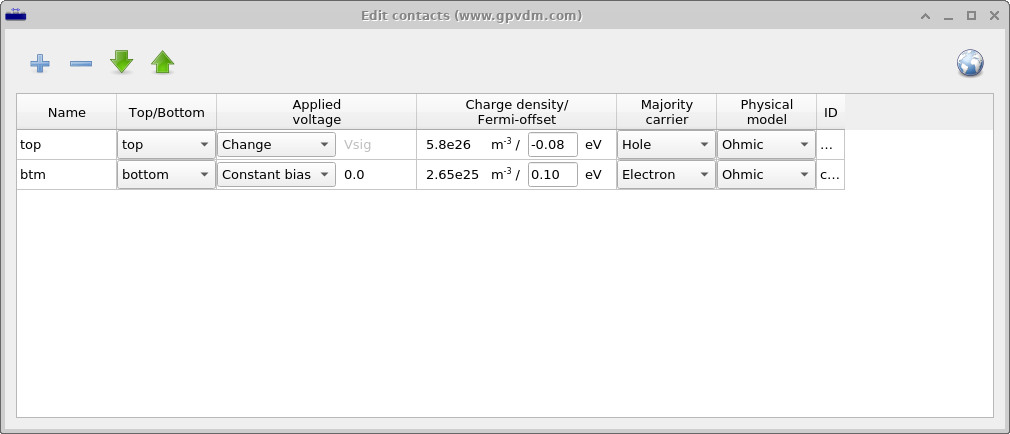
\includegraphics[width=\textwidth]{./images/contact_editor.png}
{\caption{The contact editor.}}
\label{fig:contact_editor}
\end{figure}



\subsubsection{Scanning parameters}
Sometimes one wishes to systematically vary a simulation parameter, this is how to do it:




\begin{figure}[ht!]
\centering
\includegraphics[width=\textwidth]{./images/1.jpg}
{\caption*{Step 1: Select the 'Parameter scan' tool.}}
\label{overflow}
\end{figure}


\begin{figure}[ht!]
\centering
\includegraphics[width=\textwidth]{./images/2.jpg}
\caption*{Step 2: Add a 'scan line' to the scan.}
\end{figure}

\begin{figure}[ht!]
\centering
\includegraphics[width=\textwidth]{./images/3.jpg}
\caption*{Step 3: Select the new 'scan line' and the click on the 'select parameter to change' tool.}
\label{overflow}
\end{figure}


\begin{figure}[ht!]
\centering
\includegraphics[width=\textwidth]{./images/4.jpg}
\caption*{Step 4: Select the parameter you want to change, click apply.}
\end{figure}


\begin{figure}[ht!]
\centering
\includegraphics[width=\textwidth]{./images/5.jpg}
\caption*{Step 5: The 'scan line' should now be updated with the parameter you want to scan.}
\end{figure}


\begin{figure}[ht!]
\centering
\includegraphics[width=\textwidth]{./images/6.jpg}
\caption*{Step 6: Now enter the parameters you wish to scan, in this case 0.0-0.5 suns.
Step 7: Click the run button.}
\end{figure}


\begin{figure}[ht!]
\centering
\includegraphics[width=\textwidth]{./images/7.jpg}
\caption*{Step 8: Select the output file you want to plot.  gpvdm will plot all simulation results.}
\end{figure}

\subsubsection{1D, 2D and 3D simulations with gpvdm}
When deciding if you should perform 1D, 2D or 3D, simulations, consider the dimensionality of your problem.  For example if you consider a solar cell, it is only a few micros thick, and there is rapid variation in the structure, charge densities, mobilities, and doping as a function of depth (y).  However, the structure will not vary very quickly in the lateral (xz) plane.  Therefore, in general  to capture all interesting effects present within a solar cell one only needs a 1D model.  If one now considers OFETs, there is both vertical an lateral current flow, therefore one can not get away with a 1D model any more, as one must simulate both vertical current flow, and current between the source and the drain, thus one needs a 2D simulation.  As the number of dimensions increases, computation speed will decrease, therefore my general advice is to use the minimum number of dimensions possible to solve your problem.




\newpage




\section{The user interface}
\subsubsection{Is Langevin recombination a good way of describing recombination OPV devices?}
In my view Langevin recombination is in general a really bad way to describe recombination in OPV devices.  This is because the mechanism assumes Brownian motion of electrons and holes and that charge carriers of opposite polarity will recombine when they get close enough to fall into each others electrostatic field.  This picture assumes the charge carriers are free and completely neglects the influence of trap states.  I therefore think Langeving recombination should be avoided in OPVs.
But in dx.doi.org/10.1021/jp200234m you used Langevin recombination - why?: In this paper I allowed the mobility in the Langevin expression to vary as a function of carrier density i.e.
\begin{equation}
R_{free}=q k_{r}\frac{(\alpha \mu_e(n)+\beta \mu_h(n)) n_{tot} p_{tot}}{2\epsilon_0\epsilon_r}
\end{equation}

I then by defining a mobility edge and assuming any carrier below the mobility edge could not move and any carrier above it could.  I could define the averaged electron/hole mobility as: 

\begin{equation}
\mu_e(n)=\frac{\mu_e^0 n_{free}}{n_{free}+n_{trap}}
\end{equation}

and

\begin{equation}
\mu_h(n)=\frac{\mu_h^0 p_{free}}{p_{free}+p_{trap}}
\end{equation}

and if one assumes the density of free charge carriers is much smaller than the density of trapped charge carriers one can arrive at

\begin{equation}
R(n,p)=q k_{r}\frac{(\alpha \mu_e^0 n_{free} p_{trap}+\beta \mu_h p_{free} n_{trap}) }{2\epsilon_0\epsilon_r}
\end{equation}

Thus by making the mobility carrier density dependent we arrive at an expression for Langeving recombination that's dependent upon the density of free and trapped carriers (i.e. $n_{free} p_{trap}$ and $ p_{free} n_{trap}$) This is in principle the same as SRH recombination (i.e. a process involving free electrons (holes) recombining with trapped holes (electrons)).  This was a nice simple approach and it worked quite well in the steady state.  However, to make this all work I had to assume all electrons (holes) at any given position in space had a single quasi-Fermi level, which meant they were all in equilibrium with each other.  For this to be true, all electrons (holes) would have to be able to exchange energy with all other electrons (holes) at that position in space and have an infinite charge carrier thermalization velocity.  This seemed like an OK assumption in steady state when electrons (holes) had time to exchange energy, however once we start thinking about things happening in time domain, it becomes harder to justify because there are so many trap states in the device it is unlikely that charge carriers will be able to act as one equilibrated gas with one quasi-Fermi level.  On the other hand the SRH mechanism does not make this assumption, so it is probably a better description of recombination/trapping.  I would also add that I have never found a situation in OPV device modeling where SRH recombination was unable to describe the device in question.  Conclusion: SRH is better than Langevin.  


\subsubsection{Should I trust the results of gpvdm?}
Yes!  The model it's self has been verified against experiment [there are over 20 publications doing this, in steady state, time domain (us-fs time scales), and fx-domain]. The basic drift-diffusion solver was cross checked and compared against other drift diffusion models, and the accuracy compared down to 6-9 dp.  While the optical model has been compared to analytical solutions of Maxwell's equations.  The SRH model has also been compared against analytical models.  If the answers you are getting out of gpvdm are odd, then I would suggest to take a look at the input parameters.  If your efficienceis are high, try increasing the number of trap states, the recombination cross sections or reducing the e/h mobilites.  Finally, I would also recommend always running the latest version, and keeping an eye on the twitter stream for bug announcements.



\subsection{Can I use the model to simulate my exotic* material system/contacts?}
The short answer is yes.  The model is an effective medium model, meaning that it does not simulate the details of the medium, rather it approximates the medium with a set of electrical parameters.  For example, when simulating an organic solar cell, it does not simulate every detail of the BHJ, rather it just assumes an effective mobility, density of states, recombination cross sections, trapping cross sections and so on...  So if you can find electrical parameters to aproximate your material system (or guess them), there is nothing stopping you using gpvdm to simulate any exotic device/material.  The same goes for the contacts, the model simulates the contacts simply as a charge density. So if you have fancy graphene contacts which inject lots of charge, use a high majority carrier density on the contacts.  Where as if you have some dirty old ITO contacts may be drop the majority carrier density a bit.

\newpage



\input{files}
\newpage
\section{Data privacy statement}
In some versions of gpvdm it will ask you to register before using it.  In these versions it asks for your name, title, company that you work for and what you intend on using gpvdm for.  This data is then transmitted to the gpvdm server where it is securely stored. The reason I ask for this information is to be able generate accurate usage information. Having accurate information helps when requesting grants from funding bodies.  It's much easier to ask a funding body for money if you can prove you actually have users and your software is a benefit to society. Periodicity gpvdm will also contact the gpvdm server to see if there are any software updates. By using gpvdm you agree for the above to happen.


\newpage
\section{Copyright of the manual}
This manual is released under CC-BY license.

